\documentclass{beamer}
\usepackage{amssymb}
\usepackage{graphicx}
\usepackage{wasysym}
\usetheme{Berlin}


\title[Emisi\'on de la fotosfera]{\textbf{Emisi\'on de la fotosfera}}
\author{Antonio Galv\'an}
\date{5 Mayo 2014}
\institute{Instituto de Astronom\'ia\\ Facultad
 de Ciencias\\ U.N.A.M.}

\begin{document}
\begin{frame}
\titlepage
\end{frame}

% % % % % % % % % % % % % % % % % % % % % % % % % % % % % % % % % % % % %
% % % % % % % % % % % % % Segunda diapositiva % % % % % % % % % % % % % %
% % % % % % % % % % % % % % % % % % % % % % % % % % % % % % % % % % % % % 

\begin{frame}
\frametitle{\'Indice}
\tableofcontents
\end{frame}

% % % % % % % % % % % % % % % % % % % % % % % % % % % % % % % % % % % % %
% % % % % % % % % % % % % Tercera diapositiva % % % % % % % % % % % % % %
% % % % % % % % % % % % % % % % % % % % % % % % % % % % % % % % % % % % %


\section{Introducci\'on}

\begin{frame}
\frametitle{Introducci\'on:} 
Se cree a lo largo de muchas observaciones que los GRB's surgen 
de la disipaci\'on de energ\'ia cin\'etica de un flujo relativista,
 original de un objeto central compacto.\\
Esta energ\'ia disipada es convertida en electrones energ\'eticos que
producen fotones altamente energ\'eticos por medio de radiaci\'on Sincrotron y 
Compton Inverso.
\end{frame}


% % % % % % % % % % % % % % % % % % % % % % % % % % % % % % % % % % % % %
% % % % % % % % % % % % % Cuarta diapositiva  % % % % % % % % % % % % % % 
% % % % % % % % % % % % % % % % % % % % % % % % % % % % % % % % % % % % %


\subsection{Y la fotosfera ?`qu\'e rol tiene?}
\begin{frame}
\frametitle{?`Y la fotosfera ¿qu\'e rol tiene?}
	\begin{columns}
	
		\begin{column}{5cm}
		En un modelo c\'omo lo es el termonuclear en el que propone que el material acretado
		de un sistema binario o de una estrella de neutrones peque\~na con un entorno altamente
		denso.
		\end{column}
		
		\begin{column}{5cm}
		En el modelo de la estrella de neutrones formada por una capa de hidr\'ogeno ($H$) en la capa
		m\'as externa, seguida de una capa de helio ($He$) y metales por debajo de \'esta con una densidad
		de $10^{7}g cm^{-2}$ y $T\backsim 10^{7}K $ los electrones se degeneran.\\
		De esta manera se genera una combusti\'on nuclear.
		\end{column}	
	\end{columns}
\end{frame}


% % % % % % % % % % % % % % % % % % % % % % % % % % % % % % % % % % % % %
% % % % % % % % % % % % % Quinta diapositiva  % % % % % % % % % % % % % %
% % % % % % % % % % % % % % % % % % % % % % % % % % % % % % % % % % % % %


\begin{frame}
	\begin{columns}
	
		\begin{column}{5cm}
			\begin{figure}
				\centering
				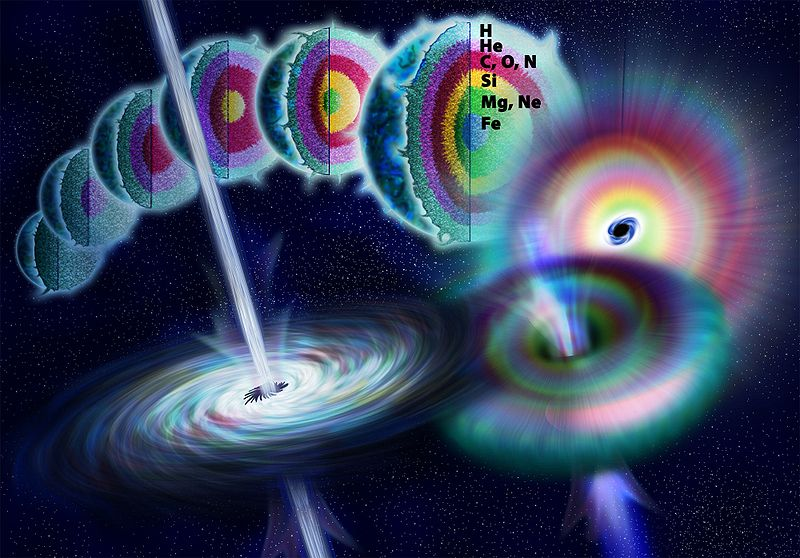
\includegraphics[scale=0.75]{neutronStar.jpg}
				\caption{Distintos procesos de la estrella de neutrones.}
			
			\end{figure}
		\end{column}
		
		\begin{column}{5cm}
		De tal forma de que el hidr\'ogeno se  por CNO no limitado y por medio de electrones 
		capturados por protones.\\ La tasa m\'inima de acreci\'on es de $\backsim 10^{15}M_{\astrosun}km^{-2}yr^{-1}$.\\
		Cu\'ando la temperatura alcanza $\backsim 10^{8}K $ la capa de $He$
		explota generando la cantidad necesaria para originar un GRB.
		\end{column}	
	\end{columns}
\end{frame}


% % % % % % % % % % % % % % % % % % % % % % % % % % % % % % % % % % % % %
% % % % % % % % % % % % % Sexta diapositiva % % % % % % % % % % % % % % %
% % % % % % % % % % % % % % % % % % % % % % % % % % % % % % % % % % % % %


\begin{frame}
	\begin{columns}
	
		\begin{column}{5cm}
		La capa de $He$ se quema de manera muy r\'apida, dentro de los $10^{-2}s$. La energ\'ia termonuclear
		se libera a la atm\'osfera y una vez ah\'i disipan su energ\'ia generando un campo el\'ectrico en \'optico.\\
		Dado que los electrones est\'an acelerados, por medio de Compton inverso producen un rayo gamma ($\gamma -ray$), con fotones
		del cuerpo negro.\\
		Estos $\gamma -ray$ de cientos de $KeV$ son intensos a trav\'es de las lineas del
		campo magn\'etico y escapan libremente por los polos.
		\end{column}	

		\begin{column}{5cm} 
			\begin{figure}
				\centering
				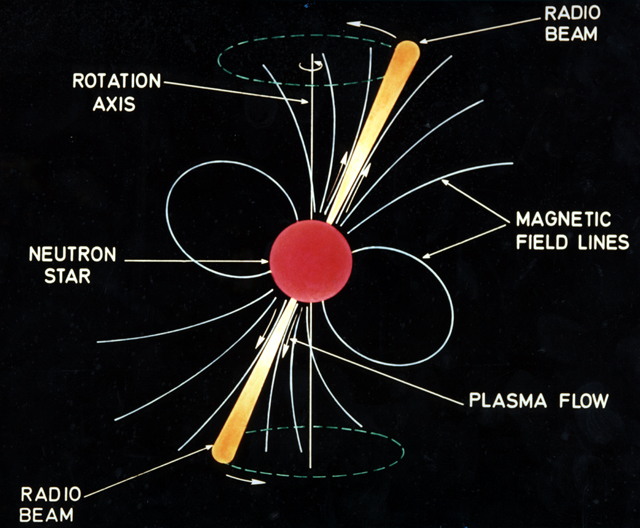
\includegraphics[scale=0.25]{expulsiondeljet.jpg}
				\caption{Observamos c\'omo toda esa energ\'ia corre libremente
				por las lineas del campo magn\'etico.}
			\end{figure}
		\end{column}	
	\end{columns}
\end{frame}


% % % % % % % % % % % % % % % % % % % % % % % % % % % % % % % % % % % % %
% % % % % % % % % % % % % Septima diapositiva % % % % % % % % % % % % % %
% % % % % % % % % % % % % % % % % % % % % % % % % % % % % % % % % % % % %



\begin{frame}
	\begin{columns}
	
		\begin{column}{5cm}
			\begin{figure}
				\centering
				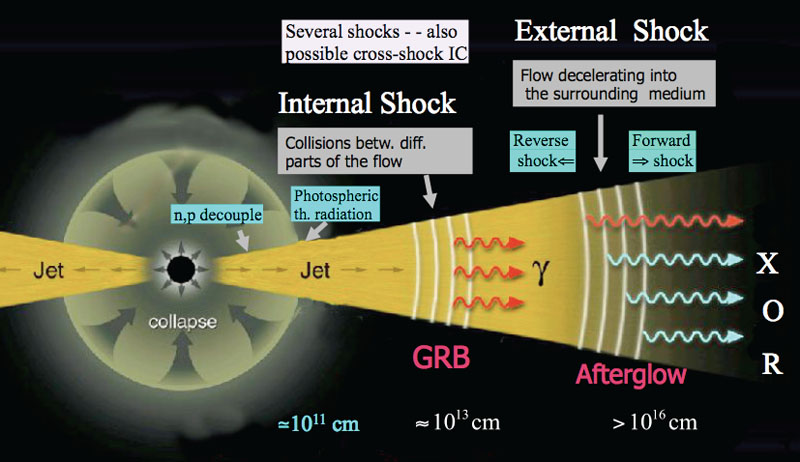
\includegraphics[scale=0.2]{figure1.jpg}
				\caption{Observemos las distancias a las que se
				genera cada momento.}
			\end{figure}
		\end{column}
		
		
		\begin{column}{5cm}
		Los fotones experimentan una dispersi\'on Compton en electrones fr\'ios y crean una subpoblaci\'on de electrones
		calientes que emiten en radiaci\'on de sincrotr\'on, que resulta ser t\'ermica y que corresponde a la energ\'ia t\'ipica
		de excitaci\'on de los electrones: $kT_{s} \backsim mc^{2}$
		\end{column}	
	\end{columns}
\end{frame}


% % % % % % % % % % % % % % % % % % % % % % % % % % % % % % % % % % % % %
% % % % % % % % % % % % % Octava  diapositiva % % % % % % % % % % % % % % 
% % % % % % % % % % % % % % % % % % % % % % % % % % % % % % % % % % % % %


\begin{frame}
	\begin{columns}
	
		\begin{column}{5cm}
		El espectro emitido por el sistema de iluminaci\'on de esta fotosfera
		es la suma de un cuerpo negro con la temperatura de algunos $KeV$ y la
		radiaci\'on de sincrotr\'on considerada c\'omo t\'ermica con temperatura
		$kT_{s} \backsim mc^{2}$. Esa energ\'ia liberada esta en el rango de 
		$10^{37} - 10^{49} erg.$ implicando distancias entre unos cientos de parsecs
		y $1-2 kpc$
		\end{column}
		
		
		\begin{column}{5cm}
		La tasa de acreci\'on siendo un flujo de rayos es de  $3 x 10^{-14}erg cm^{-2}s $.
		Para distancias de $1 kpc$ es demasiado baja para los limites deducidos por las
		observaciones de Einstein.
		
		\end{column}	
	\end{columns}
\end{frame}


% % % % % % % % % % % % % % % % % % % % % % % % % % % % % % % % % % % % %
% % % % % % % % % % % % % Novena  diapositiva % % % % % % % % % % % % % % 
% % % % % % % % % % % % % % % % % % % % % % % % % % % % % % % % % % % % %

\subsection{?`Entonces?}

\begin{frame}{?`Entonces?}
Observamos que en la fotosfera el GRB comienza a ser visible, ...

	\begin{figure}
		\centering
		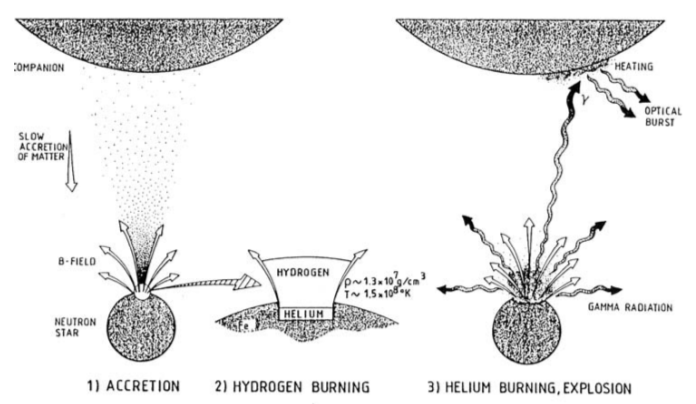
\includegraphics[scale=0.2]{creacionGRB.png}
		\caption{Ilustraci\'on del modelo termonuclear.}
	\end{figure}
\end{frame}



\end{document}
